% Options for packages loaded elsewhere
\PassOptionsToPackage{unicode}{hyperref}
\PassOptionsToPackage{hyphens}{url}
%
\documentclass[
]{article}
\usepackage{amsmath,amssymb}
\usepackage{iftex}
\ifPDFTeX
  \usepackage[T1]{fontenc}
  \usepackage[utf8]{inputenc}
  \usepackage{textcomp} % provide euro and other symbols
\else % if luatex or xetex
  \usepackage{unicode-math} % this also loads fontspec
  \defaultfontfeatures{Scale=MatchLowercase}
  \defaultfontfeatures[\rmfamily]{Ligatures=TeX,Scale=1}
\fi
\usepackage{lmodern}
\ifPDFTeX\else
  % xetex/luatex font selection
\fi
% Use upquote if available, for straight quotes in verbatim environments
\IfFileExists{upquote.sty}{\usepackage{upquote}}{}
\IfFileExists{microtype.sty}{% use microtype if available
  \usepackage[]{microtype}
  \UseMicrotypeSet[protrusion]{basicmath} % disable protrusion for tt fonts
}{}
\makeatletter
\@ifundefined{KOMAClassName}{% if non-KOMA class
  \IfFileExists{parskip.sty}{%
    \usepackage{parskip}
  }{% else
    \setlength{\parindent}{0pt}
    \setlength{\parskip}{6pt plus 2pt minus 1pt}}
}{% if KOMA class
  \KOMAoptions{parskip=half}}
\makeatother
\usepackage{xcolor}
\usepackage[margin=1in]{geometry}
\usepackage{color}
\usepackage{fancyvrb}
\newcommand{\VerbBar}{|}
\newcommand{\VERB}{\Verb[commandchars=\\\{\}]}
\DefineVerbatimEnvironment{Highlighting}{Verbatim}{commandchars=\\\{\}}
% Add ',fontsize=\small' for more characters per line
\usepackage{framed}
\definecolor{shadecolor}{RGB}{248,248,248}
\newenvironment{Shaded}{\begin{snugshade}}{\end{snugshade}}
\newcommand{\AlertTok}[1]{\textcolor[rgb]{0.94,0.16,0.16}{#1}}
\newcommand{\AnnotationTok}[1]{\textcolor[rgb]{0.56,0.35,0.01}{\textbf{\textit{#1}}}}
\newcommand{\AttributeTok}[1]{\textcolor[rgb]{0.13,0.29,0.53}{#1}}
\newcommand{\BaseNTok}[1]{\textcolor[rgb]{0.00,0.00,0.81}{#1}}
\newcommand{\BuiltInTok}[1]{#1}
\newcommand{\CharTok}[1]{\textcolor[rgb]{0.31,0.60,0.02}{#1}}
\newcommand{\CommentTok}[1]{\textcolor[rgb]{0.56,0.35,0.01}{\textit{#1}}}
\newcommand{\CommentVarTok}[1]{\textcolor[rgb]{0.56,0.35,0.01}{\textbf{\textit{#1}}}}
\newcommand{\ConstantTok}[1]{\textcolor[rgb]{0.56,0.35,0.01}{#1}}
\newcommand{\ControlFlowTok}[1]{\textcolor[rgb]{0.13,0.29,0.53}{\textbf{#1}}}
\newcommand{\DataTypeTok}[1]{\textcolor[rgb]{0.13,0.29,0.53}{#1}}
\newcommand{\DecValTok}[1]{\textcolor[rgb]{0.00,0.00,0.81}{#1}}
\newcommand{\DocumentationTok}[1]{\textcolor[rgb]{0.56,0.35,0.01}{\textbf{\textit{#1}}}}
\newcommand{\ErrorTok}[1]{\textcolor[rgb]{0.64,0.00,0.00}{\textbf{#1}}}
\newcommand{\ExtensionTok}[1]{#1}
\newcommand{\FloatTok}[1]{\textcolor[rgb]{0.00,0.00,0.81}{#1}}
\newcommand{\FunctionTok}[1]{\textcolor[rgb]{0.13,0.29,0.53}{\textbf{#1}}}
\newcommand{\ImportTok}[1]{#1}
\newcommand{\InformationTok}[1]{\textcolor[rgb]{0.56,0.35,0.01}{\textbf{\textit{#1}}}}
\newcommand{\KeywordTok}[1]{\textcolor[rgb]{0.13,0.29,0.53}{\textbf{#1}}}
\newcommand{\NormalTok}[1]{#1}
\newcommand{\OperatorTok}[1]{\textcolor[rgb]{0.81,0.36,0.00}{\textbf{#1}}}
\newcommand{\OtherTok}[1]{\textcolor[rgb]{0.56,0.35,0.01}{#1}}
\newcommand{\PreprocessorTok}[1]{\textcolor[rgb]{0.56,0.35,0.01}{\textit{#1}}}
\newcommand{\RegionMarkerTok}[1]{#1}
\newcommand{\SpecialCharTok}[1]{\textcolor[rgb]{0.81,0.36,0.00}{\textbf{#1}}}
\newcommand{\SpecialStringTok}[1]{\textcolor[rgb]{0.31,0.60,0.02}{#1}}
\newcommand{\StringTok}[1]{\textcolor[rgb]{0.31,0.60,0.02}{#1}}
\newcommand{\VariableTok}[1]{\textcolor[rgb]{0.00,0.00,0.00}{#1}}
\newcommand{\VerbatimStringTok}[1]{\textcolor[rgb]{0.31,0.60,0.02}{#1}}
\newcommand{\WarningTok}[1]{\textcolor[rgb]{0.56,0.35,0.01}{\textbf{\textit{#1}}}}
\usepackage{graphicx}
\makeatletter
\def\maxwidth{\ifdim\Gin@nat@width>\linewidth\linewidth\else\Gin@nat@width\fi}
\def\maxheight{\ifdim\Gin@nat@height>\textheight\textheight\else\Gin@nat@height\fi}
\makeatother
% Scale images if necessary, so that they will not overflow the page
% margins by default, and it is still possible to overwrite the defaults
% using explicit options in \includegraphics[width, height, ...]{}
\setkeys{Gin}{width=\maxwidth,height=\maxheight,keepaspectratio}
% Set default figure placement to htbp
\makeatletter
\def\fps@figure{htbp}
\makeatother
\setlength{\emergencystretch}{3em} % prevent overfull lines
\providecommand{\tightlist}{%
  \setlength{\itemsep}{0pt}\setlength{\parskip}{0pt}}
\setcounter{secnumdepth}{-\maxdimen} % remove section numbering
\ifLuaTeX
  \usepackage{selnolig}  % disable illegal ligatures
\fi
\usepackage{bookmark}
\IfFileExists{xurl.sty}{\usepackage{xurl}}{} % add URL line breaks if available
\urlstyle{same}
\hypersetup{
  pdftitle={Joe\_Garcia\_DATA608\_Story2},
  pdfauthor={Joe Garcia},
  hidelinks,
  pdfcreator={LaTeX via pandoc}}

\title{Joe\_Garcia\_DATA608\_Story2}
\author{Joe Garcia}
\date{2024-02-15}

\begin{document}
\maketitle

\subsection{Setup}\label{setup}

\subsection{Introduction}\label{introduction}

The Federal Reserve's mandate from Congress is to control inflation and
to maintain low unemployment. These seem to be contradictory objectives.
For this story you will need to source the following data for the last
25 years;

\subsubsection{The Consumer Price Index (CPI) (Bureau of Labor
Statistics)}\label{the-consumer-price-index-cpi-bureau-of-labor-statistics}

\subsubsection{The FED Funds Rate (FRED) (Federal Reserve
Board)}\label{the-fed-funds-rate-fred-federal-reserve-board}

\subsubsection{Unemployment Rate (Bureau of Labor
Statistics)}\label{unemployment-rate-bureau-of-labor-statistics}

\subsection{Question we have overall}\label{question-we-have-overall}

Your Data Visualizations should be designed to answer the question ``Has
the FED been able to fulfill the mandate given to it by Congress?''

\subsection{Data}\label{data}

We take 3 pieces of data from the Federal Reserve manadata to combate
unemployment. We took the 3 latest datasets from FRED website.

\begin{Shaded}
\begin{Highlighting}[]
\NormalTok{cpi\_data }\OtherTok{\textless{}{-}} \FunctionTok{read\_csv}\NormalTok{(}\StringTok{"/Users/joe/Documents/0\_CUNY\_SPS/DATA\_608\_Knowledge\_\&\_Visual\_Analytics/Story\_2/data/CPIAUCSL.csv"}\NormalTok{)}
\NormalTok{fundsrate\_data }\OtherTok{\textless{}{-}} \FunctionTok{read\_csv}\NormalTok{(}\StringTok{"/Users/joe/Documents/0\_CUNY\_SPS/DATA\_608\_Knowledge\_\&\_Visual\_Analytics/Story\_2/data/FEDFUNDS.csv"}\NormalTok{)}
\NormalTok{unemployment\_data }\OtherTok{\textless{}{-}} \FunctionTok{read\_csv}\NormalTok{(}\StringTok{"/Users/joe/Documents/0\_CUNY\_SPS/DATA\_608\_Knowledge\_\&\_Visual\_Analytics/Story\_2/data/UNRATE.csv"}\NormalTok{)}
\end{Highlighting}
\end{Shaded}

\subsection{Data Cleaning the Data}\label{data-cleaning-the-data}

We then cleaned the data, particularly we had to take the data and
create a subset so the the data could be at the same year, so that the
cpi\_data could be at the same year as the fundsrate\_data and
unemployment\_data. Then we took the subset\_fundsrate\_data and
subset\_unemployment\_data and muiltiplied them by 100 so that they
could be at they could be at the same scale as the subset\_cpi\_data.

\begin{Shaded}
\begin{Highlighting}[]
\NormalTok{subset\_cpi\_data }\OtherTok{\textless{}{-}}\NormalTok{ cpi\_data }\SpecialCharTok{\%\textgreater{}\%}
    \FunctionTok{filter}\NormalTok{(DATE }\SpecialCharTok{\textgreater{}=} \FunctionTok{as.Date}\NormalTok{(}\StringTok{"1954{-}01{-}01"}\NormalTok{) }\SpecialCharTok{\&}\NormalTok{ DATE }\SpecialCharTok{\textless{}=} \FunctionTok{as.Date}\NormalTok{(}\StringTok{"2024{-}01{-}01"}\NormalTok{))}

\NormalTok{subset\_fundsrate\_data }\OtherTok{\textless{}{-}}\NormalTok{ fundsrate\_data }\SpecialCharTok{\%\textgreater{}\%}
    \FunctionTok{filter}\NormalTok{(DATE }\SpecialCharTok{\textgreater{}=} \FunctionTok{as.Date}\NormalTok{(}\StringTok{"1954{-}01{-}01"}\NormalTok{) }\SpecialCharTok{\&}\NormalTok{ DATE }\SpecialCharTok{\textless{}=} \FunctionTok{as.Date}\NormalTok{(}\StringTok{"2024{-}01{-}01"}\NormalTok{))}

\NormalTok{subset\_unemployment\_data }\OtherTok{\textless{}{-}}\NormalTok{ unemployment\_data }\SpecialCharTok{\%\textgreater{}\%}
    \FunctionTok{filter}\NormalTok{(DATE }\SpecialCharTok{\textgreater{}=} \FunctionTok{as.Date}\NormalTok{(}\StringTok{"1954{-}01{-}01"}\NormalTok{) }\SpecialCharTok{\&}\NormalTok{ DATE }\SpecialCharTok{\textless{}=} \FunctionTok{as.Date}\NormalTok{(}\StringTok{"2024{-}01{-}01"}\NormalTok{))}


\CommentTok{\#2016{-}01{-}01}
\CommentTok{\#1954{-}01{-}01}
\NormalTok{subset\_fundsrate\_data }\OtherTok{\textless{}{-}}\NormalTok{ subset\_fundsrate\_data }\SpecialCharTok{\%\textgreater{}\%}
  \FunctionTok{mutate}\NormalTok{(}\AttributeTok{FEDFUNDS =}\NormalTok{ FEDFUNDS }\SpecialCharTok{*} \DecValTok{100}\NormalTok{)}

\NormalTok{subset\_unemployment\_data }\OtherTok{\textless{}{-}}\NormalTok{ subset\_unemployment\_data }\SpecialCharTok{\%\textgreater{}\%}
  \FunctionTok{mutate}\NormalTok{(}\AttributeTok{UNRATE =}\NormalTok{ UNRATE }\SpecialCharTok{*} \DecValTok{100}\NormalTok{)}
\end{Highlighting}
\end{Shaded}

\subsection{Data Visualizations}\label{data-visualizations}

Next, we created some graphs to visualize the data. It appears that the
Consumer Price Index (CPI) has been slowly increasing since the 1950s
and has been gradually rising more rapidly. Although there has been a
wide discrepancy between the Federal Funds Rate and the Unemployment
rate throughout history, it has been relatively stable over the last 10
years, except for the significant shock to the system in 2020 with the
job market, which was brought under control by 2024.

\begin{Shaded}
\begin{Highlighting}[]
\CommentTok{\#ggplot(subset\_cpi\_data, aes(x = DATE, y = CPIAUCSL)) +}
\CommentTok{\#  geom\_line(color = "blue") +}
\CommentTok{\#  labs(title = "Line Plot of Subsetted Data", x = "Date", y = "CPIAUCSL") +}
\CommentTok{\#  theme\_minimal()}




\FunctionTok{ggplot}\NormalTok{() }\SpecialCharTok{+}
  \FunctionTok{geom\_line}\NormalTok{(}\AttributeTok{data =}\NormalTok{ subset\_cpi\_data, }\FunctionTok{aes}\NormalTok{(}\AttributeTok{x =}\NormalTok{ DATE, }\AttributeTok{y =}\NormalTok{ CPIAUCSL, }\AttributeTok{color =} \StringTok{"Consumer Price Index"}\NormalTok{)) }\SpecialCharTok{+}
  \FunctionTok{geom\_line}\NormalTok{(}\AttributeTok{data =}\NormalTok{ subset\_fundsrate\_data, }\FunctionTok{aes}\NormalTok{(}\AttributeTok{x =}\NormalTok{ DATE, }\AttributeTok{y =}\NormalTok{ FEDFUNDS, }\AttributeTok{color =} \StringTok{"Federal FUNDS Rate"}\NormalTok{)) }\SpecialCharTok{+}
  \FunctionTok{geom\_line}\NormalTok{(}\AttributeTok{data =}\NormalTok{ subset\_unemployment\_data, }\FunctionTok{aes}\NormalTok{(}\AttributeTok{x =}\NormalTok{ DATE, }\AttributeTok{y =}\NormalTok{ UNRATE, }\AttributeTok{color =} \StringTok{"Unemployment"}\NormalTok{)) }\SpecialCharTok{+}
  \FunctionTok{labs}\NormalTok{(}\AttributeTok{title =} \StringTok{"Multiple Data Sets Featuring Federal Funds, CPI, and Unemployment"}\NormalTok{, }\AttributeTok{x =} \StringTok{"Date"}\NormalTok{, }\AttributeTok{y =} \StringTok{"Value"}\NormalTok{) }\SpecialCharTok{+}
  \FunctionTok{theme\_minimal}\NormalTok{()}
\end{Highlighting}
\end{Shaded}

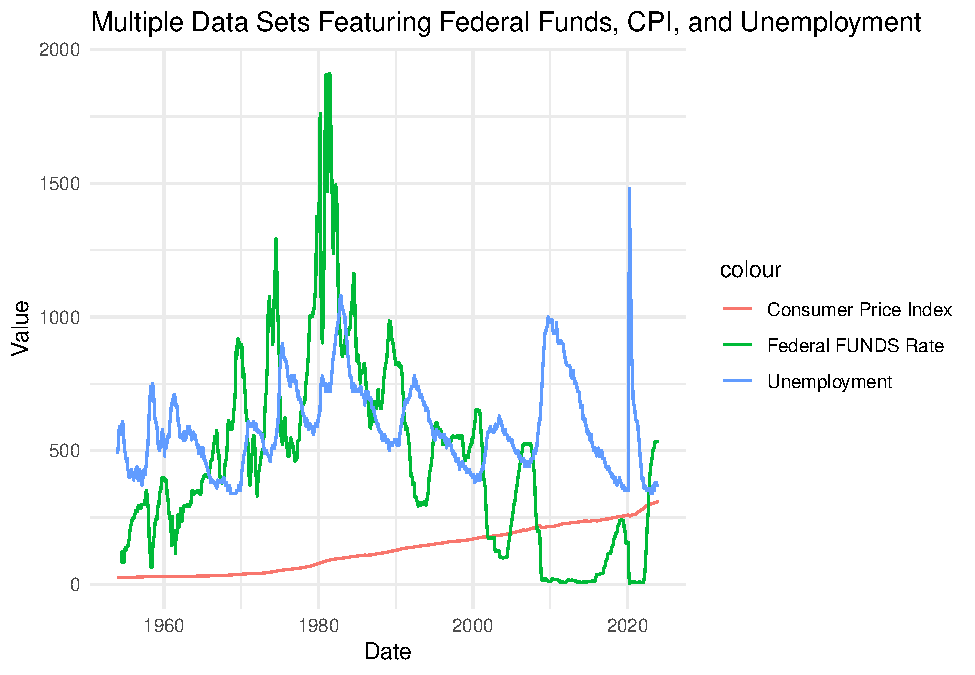
\includegraphics{Story_2_Joe_Garcia_files/figure-latex/unnamed-chunk-3-1.pdf}
\#\# Focus on the Federal Funds

Here we just look at the federal funds as the greatest to least just to
see what the range it.

\begin{Shaded}
\begin{Highlighting}[]
\NormalTok{arranged\_subset\_fundsrate\_data }\OtherTok{\textless{}{-}}\NormalTok{ subset\_fundsrate\_data }\SpecialCharTok{\%\textgreater{}\%} \FunctionTok{arrange}\NormalTok{(}\FunctionTok{desc}\NormalTok{(FEDFUNDS))}
\NormalTok{arranged\_subset\_fundsrate\_data}
\end{Highlighting}
\end{Shaded}

\begin{verbatim}
## # A tibble: 835 x 2
##    DATE       FEDFUNDS
##    <date>        <dbl>
##  1 1981-06-01     1910
##  2 1981-01-01     1908
##  3 1981-07-01     1904
##  4 1980-12-01     1890
##  5 1981-05-01     1852
##  6 1981-08-01     1782
##  7 1980-04-01     1761
##  8 1980-03-01     1719
##  9 1981-02-01     1593
## 10 1981-09-01     1587
## # i 825 more rows
\end{verbatim}

I transformed the data into merged\_data, which includes the subsets
subset\_fundsrate\_data and subset\_unemployment\_data, so that I could
create a graph with them.

\begin{Shaded}
\begin{Highlighting}[]
\NormalTok{arranged\_subset\_unemployment\_data }\OtherTok{\textless{}{-}}\NormalTok{ subset\_unemployment\_data }\SpecialCharTok{\%\textgreater{}\%} \FunctionTok{arrange}\NormalTok{(}\FunctionTok{desc}\NormalTok{(subset\_unemployment\_data))}
\NormalTok{arranged\_subset\_unemployment\_data}
\end{Highlighting}
\end{Shaded}

\begin{verbatim}
## # A tibble: 841 x 2
##    DATE       UNRATE
##    <date>      <dbl>
##  1 2024-01-01    370
##  2 2023-12-01    370
##  3 2023-11-01    370
##  4 2023-10-01    380
##  5 2023-09-01    380
##  6 2023-08-01    380
##  7 2023-07-01    350
##  8 2023-06-01    360
##  9 2023-05-01    370
## 10 2023-04-01    340
## # i 831 more rows
\end{verbatim}

\begin{Shaded}
\begin{Highlighting}[]
\NormalTok{merged\_data }\OtherTok{\textless{}{-}} \FunctionTok{inner\_join}\NormalTok{(subset\_fundsrate\_data, subset\_unemployment\_data, }\AttributeTok{by =} \StringTok{"DATE"}\NormalTok{)}
\NormalTok{merged\_data}
\end{Highlighting}
\end{Shaded}

\begin{verbatim}
## # A tibble: 835 x 3
##    DATE       FEDFUNDS UNRATE
##    <date>        <dbl>  <dbl>
##  1 1954-07-01       80    580
##  2 1954-08-01      122    600
##  3 1954-09-01      107    610
##  4 1954-10-01       85    570
##  5 1954-11-01       83    530
##  6 1954-12-01      128    500
##  7 1955-01-01      139    490
##  8 1955-02-01      129    470
##  9 1955-03-01      135    460
## 10 1955-04-01      143    470
## # i 825 more rows
\end{verbatim}

\begin{Shaded}
\begin{Highlighting}[]
\CommentTok{\#arranged\_merged\_data \textless{}{-} merged\_data \%\textgreater{}\% arrange(desc(FEDFUNDS))}
\CommentTok{\#arranged\_merged\_data}
\end{Highlighting}
\end{Shaded}

We can observe the Federal funds rate and the unemployment rate over the
same time period from 1954 to 2024. The Federal funds rate tends to
increase when the unemployment rate decreases. This relationship ideally
holds most of the time; however, there are periods where it does not
occur.

\begin{Shaded}
\begin{Highlighting}[]
\FunctionTok{ggplot}\NormalTok{(merged\_data, }\FunctionTok{aes}\NormalTok{(}\AttributeTok{x =}\NormalTok{ DATE)) }\SpecialCharTok{+}
  \FunctionTok{geom\_bar}\NormalTok{(}\FunctionTok{aes}\NormalTok{(}\AttributeTok{y =}\NormalTok{ FEDFUNDS, }\AttributeTok{fill =} \StringTok{"Fed Funds Rate"}\NormalTok{), }\AttributeTok{stat =} \StringTok{"identity"}\NormalTok{, }\AttributeTok{position =} \StringTok{"dodge"}\NormalTok{, }\AttributeTok{alpha =} \FloatTok{0.7}\NormalTok{) }\SpecialCharTok{+}
  \FunctionTok{geom\_bar}\NormalTok{(}\FunctionTok{aes}\NormalTok{(}\AttributeTok{y =}\NormalTok{ UNRATE, }\AttributeTok{fill =} \StringTok{"Unemployment Rate"}\NormalTok{), }\AttributeTok{stat =} \StringTok{"identity"}\NormalTok{, }\AttributeTok{position =} \StringTok{"dodge"}\NormalTok{, }\AttributeTok{alpha =} \FloatTok{0.7}\NormalTok{) }\SpecialCharTok{+}
  \FunctionTok{labs}\NormalTok{(}\AttributeTok{title =} \StringTok{"Comparison of Fed Funds Rate and Unemployment Rate"}\NormalTok{,}
       \AttributeTok{x =} \StringTok{"Date"}\NormalTok{,}
       \AttributeTok{y =} \StringTok{"Rate"}\NormalTok{) }\SpecialCharTok{+}
  \FunctionTok{scale\_fill\_manual}\NormalTok{(}\AttributeTok{values =} \FunctionTok{c}\NormalTok{(}\StringTok{"Fed Funds Rate"} \OtherTok{=} \StringTok{"blue"}\NormalTok{, }\StringTok{"Unemployment Rate"} \OtherTok{=} \StringTok{"red"}\NormalTok{),}
                    \AttributeTok{name =} \StringTok{"Indicator"}\NormalTok{) }\SpecialCharTok{+}
  \FunctionTok{theme\_minimal}\NormalTok{()}
\end{Highlighting}
\end{Shaded}

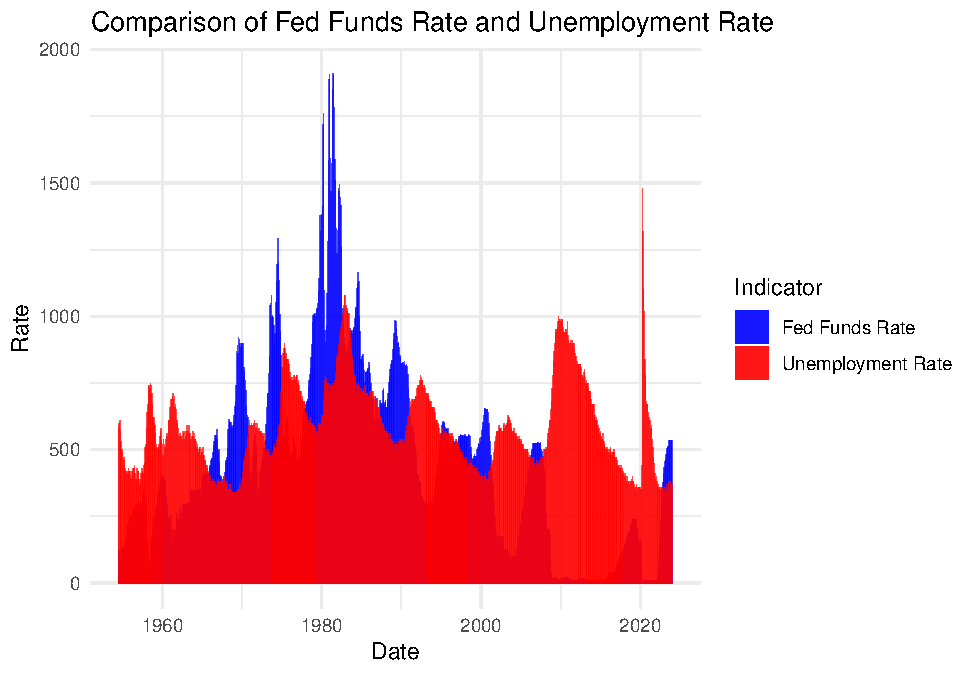
\includegraphics{Story_2_Joe_Garcia_files/figure-latex/unnamed-chunk-6-1.pdf}

Next, we placed them side by side to observe their behavior. We noted
that when the unemployment rate (in red) began to rise, the Federal
Funds Rate (in blue) also appeared to increase. However, the time period
in 2020 proved to be complicated. During this period, despite a
significant increase in unemployment, the Federal funds rate appeared to
remain stable, while the unemployment rate skyrocketed.

\begin{Shaded}
\begin{Highlighting}[]
\FunctionTok{ggplot}\NormalTok{(merged\_data, }\FunctionTok{aes}\NormalTok{(}\AttributeTok{x =}\NormalTok{ DATE)) }\SpecialCharTok{+}
  \FunctionTok{geom\_bar}\NormalTok{(}\FunctionTok{aes}\NormalTok{(}\AttributeTok{y =}\NormalTok{ FEDFUNDS, }\AttributeTok{fill =} \StringTok{"Fed Funds Rate"}\NormalTok{), }\AttributeTok{stat =} \StringTok{"identity"}\NormalTok{, }\AttributeTok{position =} \StringTok{"identity"}\NormalTok{, }\AttributeTok{width =} \DecValTok{5}\NormalTok{)}\SpecialCharTok{+}
  \FunctionTok{geom\_bar}\NormalTok{(}\FunctionTok{aes}\NormalTok{(}\AttributeTok{y =} \SpecialCharTok{{-}}\NormalTok{UNRATE, }\AttributeTok{fill =} \StringTok{"Unemployment Rate"}\NormalTok{), }\AttributeTok{stat =} \StringTok{"identity"}\NormalTok{, }\AttributeTok{position =} \StringTok{"identity"}\NormalTok{, }\AttributeTok{width =} \DecValTok{5}\NormalTok{) }\SpecialCharTok{+}
  \FunctionTok{labs}\NormalTok{(}\AttributeTok{title =} \StringTok{"Butterfly Bar Chart of Fed Funds Rate and Unemployment Rate"}\NormalTok{,}
       \AttributeTok{x =} \StringTok{"Date"}\NormalTok{,}
       \AttributeTok{y =} \StringTok{"Rate"}\NormalTok{) }\SpecialCharTok{+}
  \FunctionTok{scale\_fill\_manual}\NormalTok{(}\AttributeTok{values =} \FunctionTok{c}\NormalTok{(}\StringTok{"Fed Funds Rate"} \OtherTok{=} \StringTok{"blue"}\NormalTok{, }\StringTok{"Unemployment Rate"} \OtherTok{=} \StringTok{"red"}\NormalTok{),}
                    \AttributeTok{name =} \StringTok{"Indicator"}\NormalTok{) }\SpecialCharTok{+}
  \FunctionTok{theme\_minimal}\NormalTok{() }\SpecialCharTok{+}
  \FunctionTok{coord\_flip}\NormalTok{()}\SpecialCharTok{+}
  \FunctionTok{theme}\NormalTok{(}\AttributeTok{axis.ticks.y =} \FunctionTok{element\_line}\NormalTok{(}\AttributeTok{size =} \DecValTok{2}\NormalTok{)) }\SpecialCharTok{+}
  \FunctionTok{scale\_y\_continuous}\NormalTok{(}\AttributeTok{breaks =} \FunctionTok{seq}\NormalTok{(}\SpecialCharTok{{-}}\DecValTok{10}\NormalTok{, }\DecValTok{10}\NormalTok{, }\AttributeTok{by =} \DecValTok{1}\NormalTok{))}
\end{Highlighting}
\end{Shaded}

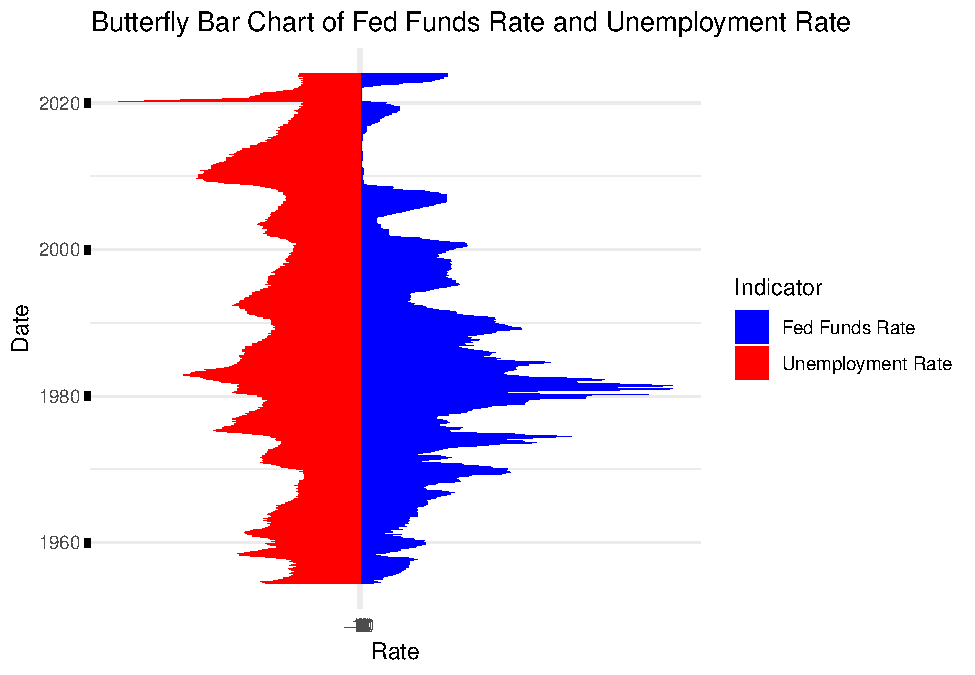
\includegraphics{Story_2_Joe_Garcia_files/figure-latex/unnamed-chunk-7-1.pdf}

We put the Federal funds rate and the unemployment rate data into array
columns in order to calculate their derivatives, which represent the
change in each column's values over time.

\begin{Shaded}
\begin{Highlighting}[]
\NormalTok{fedfunds\_array }\OtherTok{\textless{}{-}} \FunctionTok{as.array}\NormalTok{(merged\_data}\SpecialCharTok{$}\NormalTok{FEDFUNDS)}
\NormalTok{result }\OtherTok{\textless{}{-}}\NormalTok{ fedfunds\_array[}\SpecialCharTok{{-}}\DecValTok{1}\NormalTok{] }\SpecialCharTok{{-}}\NormalTok{ fedfunds\_array[}\SpecialCharTok{{-}}\FunctionTok{length}\NormalTok{(fedfunds\_array)]}

\NormalTok{unemp\_array }\OtherTok{\textless{}{-}} \FunctionTok{as.array}\NormalTok{(merged\_data}\SpecialCharTok{$}\NormalTok{UNRATE)}
\NormalTok{result2 }\OtherTok{\textless{}{-}}\NormalTok{ unemp\_array[}\SpecialCharTok{{-}}\DecValTok{1}\NormalTok{] }\SpecialCharTok{{-}}\NormalTok{ unemp\_array[}\SpecialCharTok{{-}}\FunctionTok{length}\NormalTok{(unemp\_array)]}

\NormalTok{merged\_data }\OtherTok{\textless{}{-}}\NormalTok{ merged\_data[}\SpecialCharTok{{-}}\FunctionTok{nrow}\NormalTok{(merged\_data), ]}

\NormalTok{merged\_data }\OtherTok{\textless{}{-}} \FunctionTok{cbind}\NormalTok{(merged\_data, result, result2)}
\end{Highlighting}
\end{Shaded}

\begin{Shaded}
\begin{Highlighting}[]
\CommentTok{\#ggplot(merged\_data, aes(x = DATE)) +}
\CommentTok{\#  geom\_bar(aes(y = result, fill = "Fed Funds Rate"), stat = "identity", position = "identity", width = 9)+}
\CommentTok{\#  geom\_bar(aes(y = {-}result2, fill = "Unemployment Rate"), stat = "identity", position = "identity", width = 9) +}
\CommentTok{\#  labs(title = "Butterfly Bar Chart of Fed Funds Rate and Unemployment Rate",}
\CommentTok{\#       x = "Date",}
\CommentTok{\#       y = "Rate") +}
\CommentTok{\#  scale\_fill\_manual(values = c("Fed Funds Rate" = "blue", "Unemployment Rate" = "red"),}
\CommentTok{\#                    name = "Indicator") +}
\CommentTok{\#  theme\_minimal() +}
\CommentTok{\#  coord\_flip()+}
\CommentTok{\#  theme(axis.ticks.y = element\_line(size = 2)) +}
\CommentTok{\#  scale\_y\_continuous(breaks = seq({-}50, 50, by = 1))}

\CommentTok{\#p \textless{}{-} ggplot(merged\_data, aes(x = DATE)) +}
\CommentTok{\#  geom\_line(aes(y = result, fill = "Fed Funds Rate"), stat = "identity", position = "dodge", alpha = 0.7) +}
\CommentTok{\#  geom\_line(aes(y = {-}result2, fill = "Unemployment Rate"), stat = "identity", position = "dodge", alpha = 0.7) +}
\CommentTok{\#  labs(title = "Comparison of Fed Funds Rate and Unemployment Rate",}
\CommentTok{\#       x = "Date",}
\CommentTok{\#       y = "Rate") +}
\CommentTok{\#  scale\_fill\_manual(values = c("Fed Funds Rate" = "blue", "Unemployment Rate" = "red"),}
 \CommentTok{\#                   name = "Indicator") +}
\CommentTok{\#  theme\_minimal()}

\CommentTok{\#p + ylim({-}250,250)}

\CommentTok{\#dates \textless{}{-} as.array(merged\_data$DATE)}
\CommentTok{\#dates \textless{}{-} dates[{-}length(dates)]}

\CommentTok{\#merged\_data \textless{}{-} data.frame(dates, result, result2)}
\end{Highlighting}
\end{Shaded}

\begin{Shaded}
\begin{Highlighting}[]
\NormalTok{merged\_data }\OtherTok{\textless{}{-}}\NormalTok{ merged\_data[merged\_data}\SpecialCharTok{$}\NormalTok{DATE }\SpecialCharTok{\textgreater{}} \FunctionTok{as.Date}\NormalTok{(}\StringTok{"2016{-}01{-}01"}\NormalTok{), ]}

\CommentTok{\#p\textless{}{-} ggplot() +}
\CommentTok{\#  geom\_line(data = merged\_data, aes(x = DATE, y = result, color = "Federal Funds")) +}
\CommentTok{\#  geom\_line(data = merged\_data, aes(x = DATE, y = {-}result2, color = "Unemployment")) +}
\CommentTok{\#  labs(title = "Line Chart with Multiple Data Sets", x = "Date", y = "Value") +}
\CommentTok{\#  theme\_minimal()}
\CommentTok{\#p + ylim({-}100,100)}

\NormalTok{p }\OtherTok{\textless{}{-}} \FunctionTok{ggplot}\NormalTok{(merged\_data, }\FunctionTok{aes}\NormalTok{(}\AttributeTok{x =}\NormalTok{ DATE)) }\SpecialCharTok{+}
  \FunctionTok{geom\_bar}\NormalTok{(}\FunctionTok{aes}\NormalTok{(}\AttributeTok{y =}\NormalTok{ result, }\AttributeTok{fill =} \StringTok{"Fed Funds Rate"}\NormalTok{), }\AttributeTok{stat =} \StringTok{"identity"}\NormalTok{, }\AttributeTok{width =} \DecValTok{30}\NormalTok{, }\AttributeTok{alpha =} \FloatTok{0.5}\NormalTok{) }\SpecialCharTok{+}
  \FunctionTok{geom\_bar}\NormalTok{(}\FunctionTok{aes}\NormalTok{(}\AttributeTok{y =} \SpecialCharTok{{-}}\NormalTok{result2, }\AttributeTok{fill =} \StringTok{"Unemployment Rate"}\NormalTok{), }\AttributeTok{stat =} \StringTok{"identity"}\NormalTok{, }\AttributeTok{width =} \DecValTok{30}\NormalTok{, }\AttributeTok{alpha =} \FloatTok{0.5}\NormalTok{) }\SpecialCharTok{+}
  \FunctionTok{labs}\NormalTok{(}\AttributeTok{title =} \StringTok{"Comparison of Fed Funds Rate and Unemployment Rate"}\NormalTok{,}
       \AttributeTok{x =} \StringTok{"Date"}\NormalTok{,}
       \AttributeTok{y =} \StringTok{"Rate"}\NormalTok{) }\SpecialCharTok{+}
  \FunctionTok{scale\_fill\_manual}\NormalTok{(}\AttributeTok{values =} \FunctionTok{c}\NormalTok{(}\StringTok{"Fed Funds Rate"} \OtherTok{=} \StringTok{"blue"}\NormalTok{, }\StringTok{"Unemployment Rate"} \OtherTok{=} \StringTok{"red"}\NormalTok{),}
                     \AttributeTok{name =} \StringTok{"Indicator"}\NormalTok{) }\SpecialCharTok{+}
  \FunctionTok{theme\_minimal}\NormalTok{()}
\NormalTok{p }\SpecialCharTok{+} \FunctionTok{ylim}\NormalTok{(}\SpecialCharTok{{-}}\DecValTok{100}\NormalTok{, }\DecValTok{100}\NormalTok{)}
\end{Highlighting}
\end{Shaded}

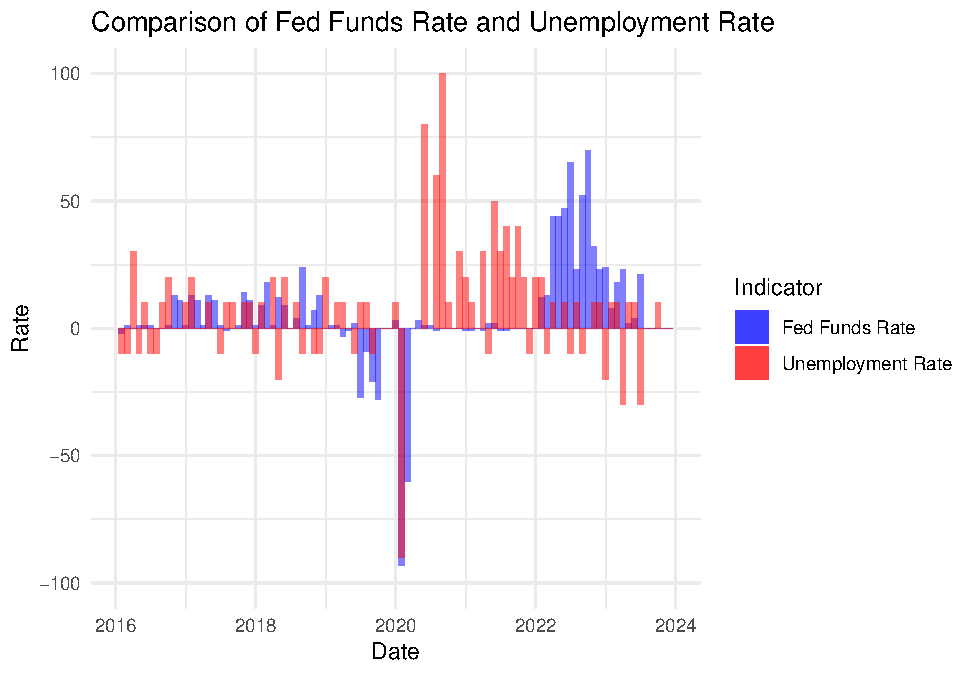
\includegraphics{Story_2_Joe_Garcia_files/figure-latex/unnamed-chunk-10-1.pdf}

\subsection{Conclusion}\label{conclusion}

Has the Fed been able to fulfill the mandate given to it by Congress?
Based on the visual analysis of the data we obtained from FRED, it
appears that the Federal Reserve has been successful in reducing the
unemployment rate through its management of the federal funds rate.
Therefore, I believe they have fulfilled the mandate given to them by
Congress.

\end{document}
